%This section introduces our new vision of data integration, proposes our approach and briefly presents our query rewriting algorithm guided by user preferences and SLAs.

%\subsection{New vision of Data Integration}
%In our work, we consider a new vision of data integration in a multi-cloud context (see figure~\ref{fig:scenario}).
Figure~\ref{fig:scenario} illustrates our vision of data integration. Data are accessed and retrieved as \textit{data services} deployed in \textit{cloud providers} geographically distributed. \textit{Data services} and \textit{cloud providers} export their SLA specifying the level of services they can guarantee to users. Two types of SLA are considered: (1) cloud SLA (SLA$_{C}$), agreements between a \textit{data service} and a \textit{cloud provider}; and (2) service SLA (SLA$_{S}$), agreements between \textit{users} and \textit{data services}. The figure~\ref{fig:cloudsla} illustrates the cloud SLA schema used by our approach. The schema includes five groups describing (i) general information concerning the agreed service and parties; (ii) business rules (such as billing method, contract validity period, price, penalties and violations); and (iii) guarantees in terms of performance, security and data management.  

\begin{figure}[th!]
\center
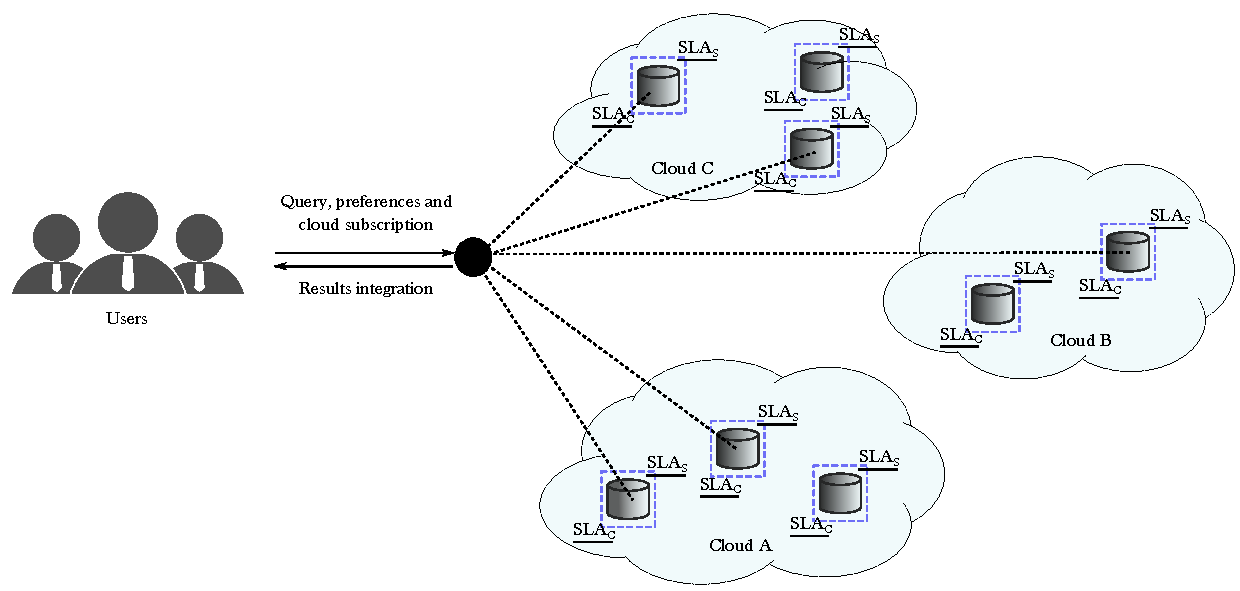
\includegraphics[scale=0.40]{scenario.pdf}
\caption{Data integration scenario}\label{fig:scenario}
\end{figure}

\begin{figure*}[th!]
\center
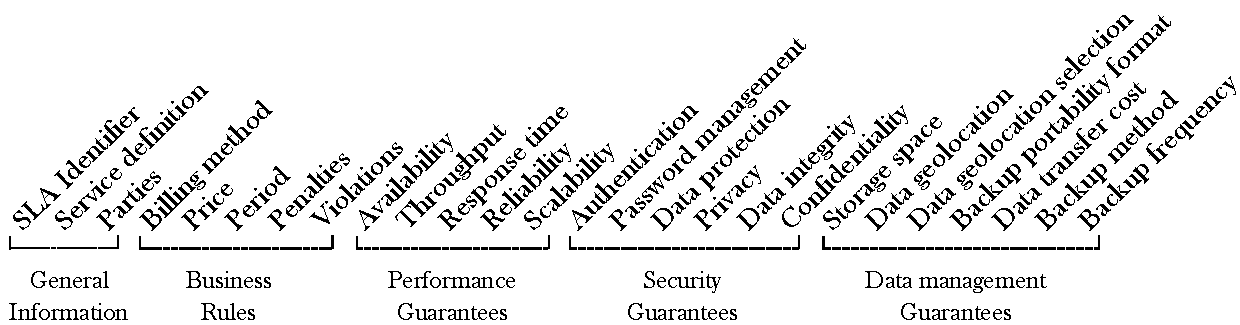
\includegraphics[scale=0.57]{Cloud_SLA.pdf}
\caption{Cloud SLA model}\label{fig:cloudsla}
\end{figure*}

Therefore, given a user query, his/her integration quality requirements and cloud subscription, the query is rewritten in terms of cloud services (\textit{data services} and \textit{data processing services}) composition that fulfill the integration requirements and deliver the expected results to the user. This new vision brings challenges to data integration, such as: (i) \underline{Performance issues}. Given the huge amount of \textit{data services}, \textit{data processing services} present in the multi-cloud context, the data integration tasks can require a huge amount of cloud resources and processing time; (ii) \underline{Economic model}. Even with the on-demand and pay-per-use imposed by the cloud, users are limited to the resources they have contracted and to the budget they are ready to pay for while asking for a integration. %\underline{Economic model}. The cloud provides resources in an on-demand and pay-per-use way to cloud consumers. However they are limited to the resources they have contracted and to the budget they are ready to pay for. 
%Thus, it is crucial to design new methods for data integration adapted to this new context; 
(iii) \underline{Quality issues}. Some rewritings produced and executed to the user query could not satisfy his/her quality requirements concerning privacy, data provenance, cost, among others. Consequently, users may become dissatisfied with the obtained results; (iv) \underline{SLA heterogeneity}. In the multi-cloud, \textit{cloud services} and \textit{cloud providers} export their SLAs with different semantics and structure making the matching of users' integration requirements with the SLAs more challenging. Moreover, while integrating services, we can also face incompatibilities of SLAs such as measures with the same meaning but with different names, measures with the same name but with different associated values and units, among others; and (iv) \underline{Reuse}. Rewriting and executing the user query is computationally costly in terms of processing time and economic cost. Thus, it is necessary to propose a manner of reusing previous integration in order to save time and money, but also meeting the user expectations.
%\bigskip

Motivated by these challenges, our data integration approach adapted to the multi-cloud is detailed in the next sections.


%\begin{itemize}
%\item \textbf{Performance}. In the multi-cloud, we are dealing with a huge amount of \textit{data services}, \textit{data processing services} and \textit{cloud providers}. Consequently, producing and executing service compositions can require an important quantity of resources and processing time.
%\item \textbf{Economic model}. Even with the possibility of having an unlimited access to resources, the user is limited to the resources he/she has contracted and to the budget he/she is ready to pay for. Thus, it is crucial to design new methods in order to produce rewritings which satisfies the user integration requirements and the cloud economic model. 
%\item \textbf{Quality issues}. Some rewritings produced and executed to the user query could not satisfy her quality requirements concerning privacy, data provenance, cost, among others. Producing and executing these rewritings implies increasing time processing and integration total cost. 
%\item \textbf{SLA heterogeneity}. In the multi-cloud, \textit{cloud services} and \textit{cloud providers} export their SLAs with different semantics and structure making the matching of users' integration requirements with the SLAs more challenging. Moreover, while integrating services, we can also face incompatibilities of SLAs such as measures with the same meaning but with different names, measures with the same name but with different associated values and units, among others.
%%\item \textbf{SLA heterogeneity}. While producing the rewritings, it is necessary to match the user requirements with the different SLAs exported by the \textit{cloud providers} and \textit{cloud services}. In the multi-cloud, \textit{cloud providers} and \textit{cloud services} export SLAs with different semantics and structure that makes the matching SLA and user requirement challenging. In addition, we are also dealing with incompatibilities of SLAs.
%\item \textbf{Reuse}. Rewriting and executing the user query is computationally costly in terms of processing time and economic cost. Thus, it is necessary to propose a manner of reusing previous integration in order to save time and money, but also meeting the user expectations.
%\end{itemize}

\subsection{SLA-based data integration}
We propose our SLA-based data integration approach which includes (i) looking for services that can be used as \textit{data services} and \textit{data processing services}, the last are responsible to retrieve and integrate data; (ii) data retrieval and integration; and (iii) delivering results to the user considering context and resource consumption.  In this sense, our approach is divided in four steps as illustrated in the figure~\ref{fig:generalapproach}. 
\begin{figure}[h!]
\centering
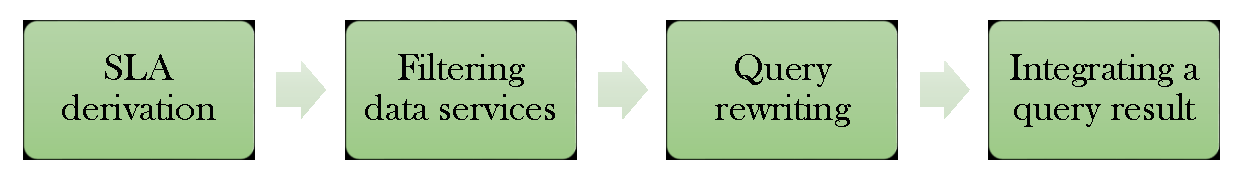
\includegraphics[scale=0.4]{workflow-approach.pdf}
\caption{SLA-based data integration workflow.}
\label{fig:generalapproach}
\end{figure}

Given a user \textit{query}, a set of associated user \textit{preferences}, \textit{cloud providers} and \textit{cloud services}:
\\
\textbf{\underline{SLA derivation}}. In this step, we compute what we call an \textsl{derived SLA} that matches user' integration requirements (including quality constraints and data requirements) with the SLA's provided by \textit{cloud services}, given a specific user cloud subscription. The user may have general \textit{preferences} depending on the context she wants to integrate her data such as economic cost, bandwidth limit, free services, and storage and processing limits. The \textit{SLA derivation} is the big challenge while dealing with SLAs and particularly for adding quality dimensions to data integration. Furthermore, the \textsl{derived SLA} guides the query evaluation, and the way results are computed and delivered. \\
\textbf{\underline{Filtering data services}}. The \textsl{derived SLA} is used (i)
to filter previous \textsl{integration SLA} derived for a similar request in order to reuse results; or (ii) to filter possible \textit{cloud services} that can be used for answering the query. \\ %The SLA exported by a selected \textit{cloud service} should satisfy the user \textit{preferences}. \\
\textbf{\underline{Query rewriting}}. Given a set of \textit{data services} that can
potentially provide data for integrating the query result, a set of service compositions is generated according to the \textsl{derived SLA} and the agreed SLA of each \textit{data services}. \\
\textbf{\underline{Integrating a query result}}. The service compositions are
executed with services from one or several clouds where the user has a
subscription.
The execution cost of service compositions must fulfill the \textsl{derived
SLA}. The clouds resources needed by the user to execute the composition and how
to use them is decided taking in consideration the economic cost determined by
the data to be transferred, the number of external calls to services, data storage and delivery cost.

The algorithm 1 describes in general lines our approach which integrate data
from multi-cloud environments considering quality aspects.
%
As input, we consider (1) a user query $Q$; (2) a set of user preferences $P$;
(3) a user cloud subscription $C$; (4) a set of previous \textit{integrated SLA}
$\bigSLA$, obtained from a local register; (5) a set of \textit{data services}
$DS$; (6) a set of \textit{data processing services} $DPS$; and (7) a set of \textit{cloud providers} $CP$. As output, the integration results $IR$ is delivered to the user while fulfilling her preferences and cloud subscription.
%

The approach begins looking for previous \textit{integrated SLAs} in our
local registry. From each \textit{integrated SLA} we verify if it matches
the user' query and preferences (lines 2 - 6), and adding them to the set $pI$ (line 4).
%
If previous \textit{integrated SLA} matches (line 7), the one that
partially matches with the user preferences is selected (line 8).
%
Then, a new \textit{integrated SLA} is computed for user query based on the
previous \textit{integrated SLA}, her preferences and cloud subscription (line 9).
%
The service compositions produced to a previous query is reused based its \textit{integrated SLA} ($sI$). 
%
Otherwise, a new \textit{integrated SLA} is created to user request given the query, her preferences and cloud subscription (line 11). 
%
The SLA information of $\mathit{DS}$ and $\mathit{DPS}$ is extracted and included in the set of \bigS (line 12). 
%
This new \textit{integrated SLA} is updated by calling the \textit{Rhone} procedure (line 13). 
%
The \textit{Rhone} is responsible of (i) selecting \textit{data services} (in $DS$) and \textit{data processing services} (in $DPS$) which satisfy the user preferences based on their SLAs; and (ii) producing service compositions that completely match with the query and fulfill the user preferences. 
%
Finally, the integration results ($IR$) are produced and delivered to the user considering her cloud subscription. 
%
Note that while executing compositions, it is necessary to satisfy the user requirements and cloud subscription, and also to dynamically update the \textit{integrated SLA} adding the information of contracts that were established to allow the integration. 
%
Finally, the \textit{integrated SLA} is stored in our registry to be used in a next query.   

\begin{algorithm} 
%\small
\caption{ - SLA-based data integration}
\label{qualityBasedAlgorithm}
\begin{algorithmic}[1]
\REQUIRE Query ($Q$), user preferences ($P$), user cloud subscriptions ($C$), a
set of \textit{data services} ($\mathit{DS}$) and \textit{data processing services} ($\mathit{DPS}$) and a set of previous \textit{integrated SLA} ($\bigSLA$).
\ENSURE Integration results delivered considering the user cloud subscription.
%\STATE \textbf{function} $\mathit{SelectCandidateServices} (Q, \bigS)$
%\STATE let $\bigSLA$ be a set of previous integrated SLA
\STATE $pI \leftarrow \emptyset$
\FORALL  {$SLA_{i}$ in $\bigSLA$}
	\IF {$\mathit{macthes(Q, P, SLA_{i})}$}
		\STATE $pI \leftarrow pI \cup \lbrace SLA_{i} \rbrace$		
%		\FORALL  {$A_{j}$ in $S_{i}$}
%			\IF {$Q.\mathit{notContains(A_{i})}$}
%				\STATE $b \leftarrow \mathit{false}$	
%				\STATE $\mathit{break}$
%			\ENDIF
%		\ENDFOR
%		\IF {$b = true$}
%			\STATE $\bigLS \leftarrow \bigLS \cup \lbrace S_{i} \rbrace$	
%		\ENDIF
	\ENDIF
\ENDFOR
\IF {$pI \neq \emptyset$}
	\STATE $sI \leftarrow chooseBest(P, pI)$
	\STATE $newSLA_{i} \leftarrow deriveSLA(sI, P, C)$
%	\FORALL  {$SLA_{i}$ in $pI$}
%		\STATE $sI \leftarrow choose(P,)$
%	\ENDFOR
\ELSE
	\STATE $newSLA_{i} \leftarrow deriveSLA(Q, P, C)$
	\STATE $\bigS \leftarrow extract(\mathit{DS}, \mathit{DPS})$
	\STATE $newSLA_{i} \leftarrow updateSLA(Rhone(Q, \bigS))$
\ENDIF
\STATE $IR \leftarrow execute(newSLA_{i})$
\STATE \textbf{return} $IR$
\STATE \textbf{end function}
\end{algorithmic}
\end{algorithm} 

\subsection{SLA-based query rewriting algorithm}
To serve a proof of concept to our approach, we develop a query
rewriting algorithm which is guided by users' integration requirements and
service level agreements exported by different data services and cloud
providers. Researches have refered to data integration as a service composition problem
in which given a query the objective is to lookup and compose data services that
can contribute to produce a result. Currently, we have formalized and developed a rewriting
algorithm that considers user preferences and services' quality aspects while
selecting services and producing rewritings called \textit{Rhone} (See algorithm
\ref{algo-rhone}, invoked in the algorithm 1, line 12).
The \textit{Rhone} algorithm consists in four macro steps: 
\\
\textbf{\underline{Selecting data services}}. The \textit{Rhone} looks for
\textit{data services} (line 2) that can contribute to answer the query while
satisfying the user' preferences; \\
\textbf{\underline{Building candidate service descriptions}}. A candidate
service description (CSD) describes how a \textit{data service} can contribute to answer the query. CSD maps a \textit{data service} (including its variables) to the entire query or part of it. For all selected services, the \textit{Rhone} tries to build CSDs when the mapping of variables is possible (line
3). \\
\textbf{\underline{Combining CSDs}}. All CSDs are combined (line 4) producing a
list of CSD combinations. Each combination can be a rewriting of the query. \\
\textbf{\underline{Producing rewritings}}. Each list of CSDs is checked in order
to verify whether it is a rewriting of the query or not (line 9). To be a
valid rewriting, it is forbidden to have CSDs covering the same part of the query.
Rewritings are produced while the user' requirements are being respected (lines 6-14).
%
The originality of our algorithm concerns the functions ~\!\tqI{}, ~\!\tqT{} and ~\!\tqS{}.     
They are responsible to initialize, check and increment user preferences
associated to some aggregation like user constraints (total cost). This means
that these preferences are initialized (line 6), and for each element in the CSD list they are incremented (line 11), and rewritings are produced while they are respected (line 8).  The result of this step is the list of valid rewritings of the query (line 14).

\begin{algorithm}
\small
\caption{ - \textit{Rhone}}
\label{algo-rhone}
\begin{algorithmic}[1]
\REQUIRE A query $Q$, a set of user preferences, and a set of concrete services $\bigS$.
\ENSURE A set of rewritings $R$ that matches with the query and fulfill the user preferences.
\STATE \textbf{function} $\mathit{Rhone} (Q, \bigS)$
 \STATE  $\bigLS \leftarrow \mathit{SelectCandidateServices}(Q, \bigS)$ \label{rhone:buildPCD}
 \STATE  $\bigLCSD \leftarrow CreateCSDs(Q, \bigLS)$
 \STATE  $I \leftarrow CombineCSDs(\bigLCSD)$
 \STATE $R\leftarrow \emptyset$
 \STATE ~\!\tqI{\agg{Q}} 
    \STATE $p \leftarrow I.next()$
    \WHILE {$p\ \neq\ \emptyset$ \AND ~\!\tqT{\agg{Q}}} 
      \IF {\textit{isRewriting}$(Q, p)$}
  \STATE $R\leftarrow R\,\cup \mathit{Rewriting}(p)$
  \STATE ~\!\tqS{\agg{Q}}
   \ENDIF
      \STATE $p \leftarrow I.\mathit{next}()$
 \ENDWHILE
    \STATE \textbf{return} $R$
\STATE \textbf{end function}
\end{algorithmic}
\end{algorithm}
%
%To serve as a proof of concept to our approach, we intend to develop a query
%rewriting algorithm which is guided by users' integration requirements and
%service level agreements exported by different data services and cloud
%providers. The query rewriting is an important issue in data integration. In
%cloud computing, researches have refereed to it as a service composition problem
%in which given a query the objective is to lookup and compose data services that
%can contribute to produce a result. \cite{Barhamgi2010} proposed a query
%rewriting approach which processes queries on data provider services.
%\cite{Benouaret2011} introduced a service composition framework to answer
%preference queries. Two algorithms inspired on~\cite{Barhamgi2010} are presented
%to rank the best rewritings based on previously computed scores. \cite{ba2014}
%extended \cite{Umberto} and presented an refinement algorithm that produces and
%order rewritings according to user preferences and scores. In general, these
%works share the same performance problem depending on the size of the query and
%on the number of available services. Furthermore, they do not take into
%consideration user's integration requirements what can lead to produce
%rewritings that are not satisfactory to the user in terms of quality
%requirements and cost. Currently, we have formalized and developed a rewriting
%algorithm that considers user preferences and services' quality aspects while
%selecting services and producing rewritings called \textit{Rhone} (Invoked in the algorithm 1, line 12).                     